
The power spectral density of a wide-sense stationary process, $X_t$, is defined as follows:
\begin{align}
    S(f) & = \int_{-\infty}^{\infty}R(\tau)e^{-2\pi\imath f \tau}d\tau, \label{eq:psdauto} \index{power spectral density}
\end{align}
where $R$ is the (non-central) autocovariance\index{autocovariance} function of $X_t$: $R(\tau)=E[X_{t+\tau} X_t]$.  For ergodic processes, where the ensemble average is equal to the time-average, the PSD can be expressed as
\begin{align}
    S(f) & = \lim_{T\to\infty}E\left[\frac{1}{T}\|\mathcal{F}_T(x)(f)\|^2\right], \label{eq:psdfourier}
\end{align}
where $\mathcal{F}_T$ is the finite-time Fourier transform operator on the time-interval $[0,T]$, and $x(t)$ is a realization of the process $X_t$.  The first definition, Equation \eqref{eq:psdauto}, requires complete knowledge of the autocovariance function $R(\tau)$.  The second, Equation \eqref{eq:psdfourier}, requires a realization of $X_t$ to be known for all time.  It seems to determine the spectrum of a process, one needs an infinite amount of information. 

\subsection{The Periodogram}

In most practical applications, the only information available are discrete measurements of one realization of a process over a finite time interval.  This leads to the simplest and most famous of the non-parametric spectrum estimators: the Periodogram\index{periodogram},
\begin{align}
    \hat{S}^{(p)}(f) & = \frac{1}{T}\|\mathcal{F}_T(x)(f)\|^2.
\end{align}
If the process is only known at a discrete set of points, the Fourier transform can be replaced by a discrete Fourier transform (DFT).  As long as the Nyquist conditions are met, this substitution results in no loss of information.  In what follows, the frequency variable is assumed to be normalized such that $f\in[-1/2,1/2]$.  

The expected value of the periodogram is related to the true spectrum, $S$, through the following equation \cite{percival:multitaper}:
\begin{align}
    E\left[\hat{S}^{(p)}(f)\right] & = \int_{-1/2}^{1/2}F_N(f-f^\prime)S(f^\prime)df^\prime,
\end{align}
where $F_N$ is Fej\'er's kernel,
\begin{align*}
    F_N(f) & = \dfrac{\sin^2(N \pi f)}{ N \sin^2(\pi f) }.\index{Fej\'er's kernel}
\end{align*}
Thus, the periodogram can be viewed as a smeared version of the true spectrum, where the smearing function is described by Fej\'er's kernel.  An example of this kernel for $N=64$ is shown in Figure \ref{fig:fejer}.  The main lobe causes peaks in the true spectrum to be smeared locally, which limits the resolution of the estimate.  The side-lobes (which seem to level-off at -20 dB) cause leakage, which introduces a broad-band bias\index{broad-band bias} across the estimate.  The leakage (and hence, bias) can be reduced by somehow reducing the height of the side-lobes.  This can be achieved with the use of a data taper.

\begin{figure}
    \centering
    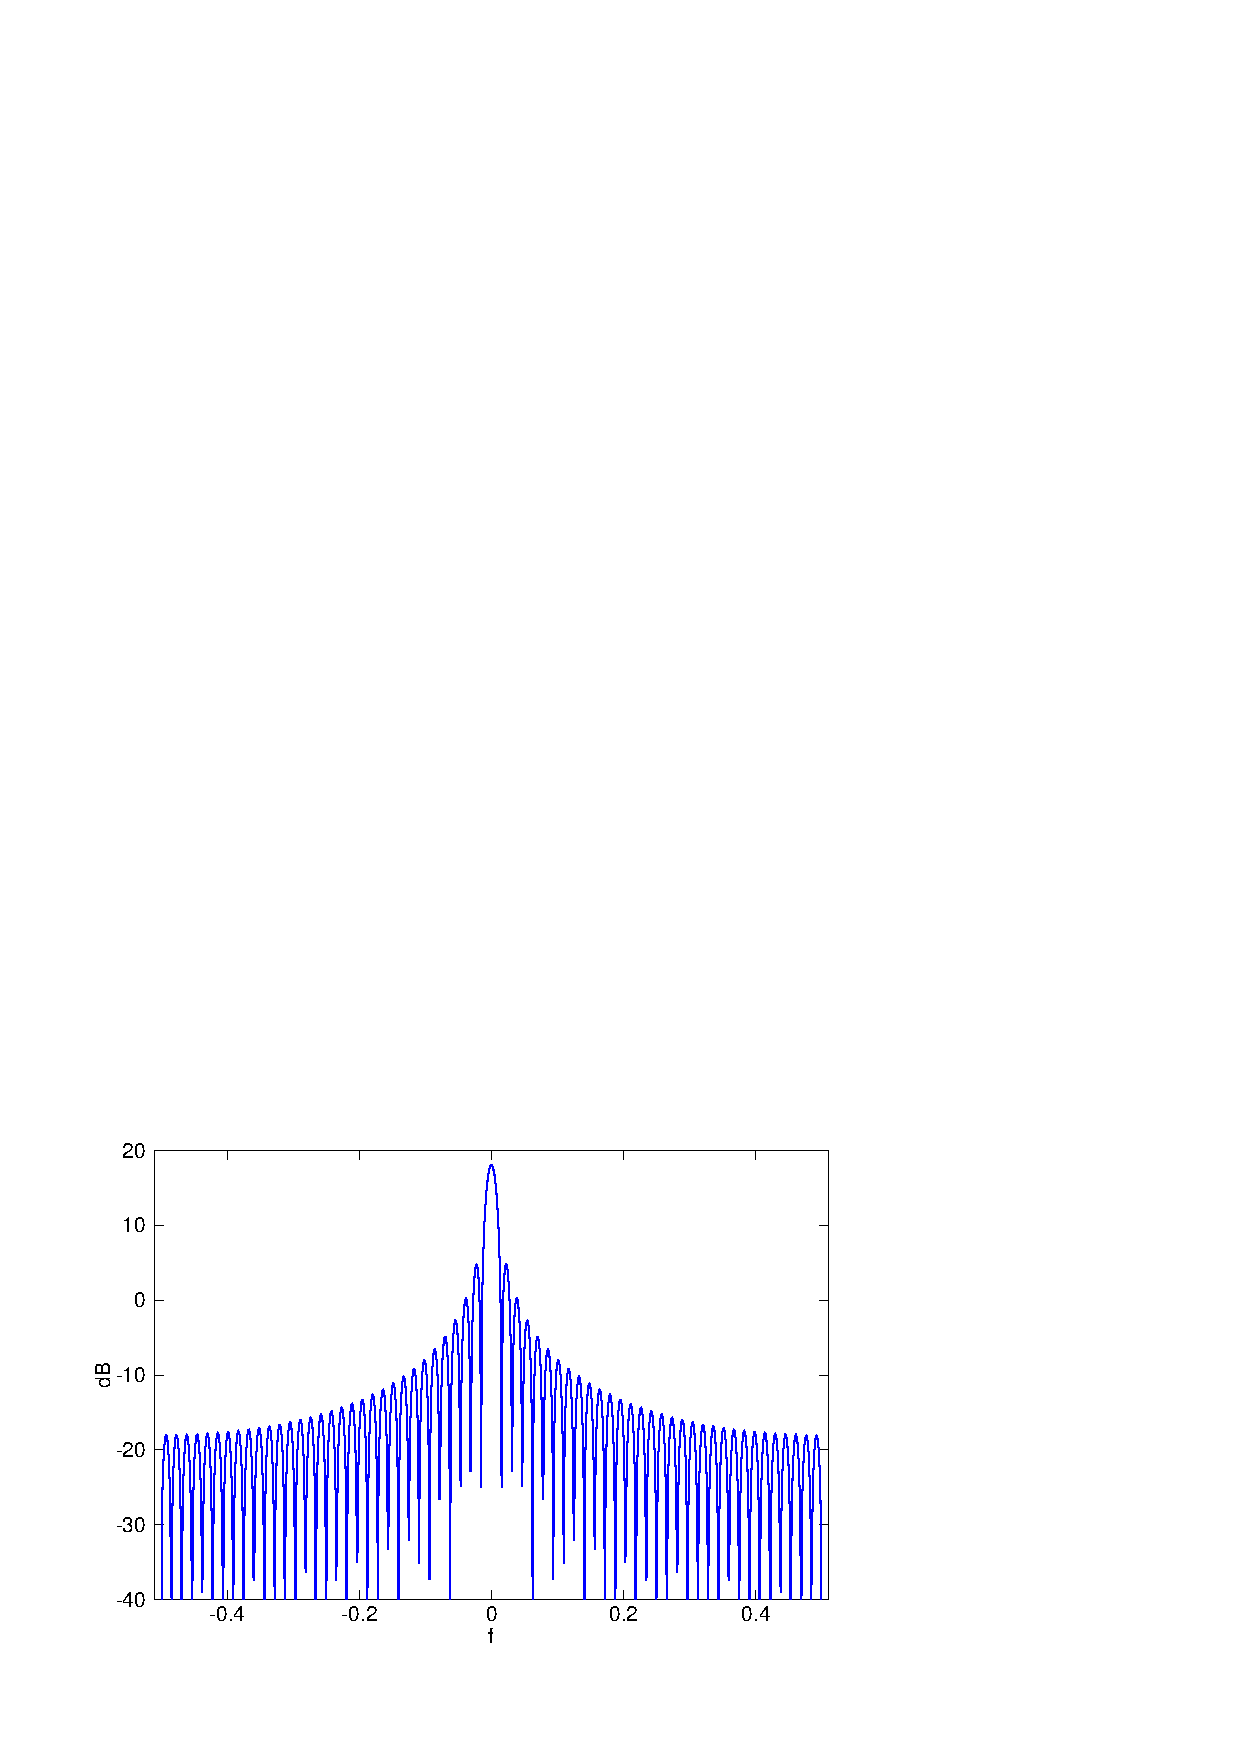
\includegraphics[width=4.5in]{pics/fejer64.pdf}
    \caption[Fej\'er's kernel]{Fej\'er's kernel, N=64 \label{fig:fejer}}
\end{figure}

\subsection{Data Tapers \label{sec:tapers}}

It can be shown that if the data is first windowed (or tapered) by a function, $\tilde{x}(t)=h(t)x(t)$, then the periodogram of this windowed function is related to the true spectrum:
\begin{align}
    \hat{S}^{(d)}(f) & = \frac{1}{T}\|\mathcal{F}(\tilde{x})(f)\|^2, & E\left[\hat{S}^{(d)}(f)\right] & = \int_{-1/2}^{1/2}H(f-f^\prime)S(f^\prime)df^\prime,
\end{align}
where $H=\|\mathcal{F}(h)\|^2$.  $\hat{S}^{(d)}$ is what Percival and Walden \cite{percival:multitaper} refer to as a direct spectral estimator\index{direct spectral estimator}.  It remains to select an ideal taper, $h$.  Such an ideal taper must have finite support in time (in order to be applied to the finite measurements $x$), and would minimize the height of the side-lobes in the frequency domain.  

David Slepian at Bell Labs studied such concentration problems, and developed what are now known as the discrete prolate spheroidal sequences (DPSSs) \cite{slepian:seq}.  They are sometimes referred to as Slepian sequences in his honour.  The discrete version of the concentration problem is as follows:
\smallskip

\begin{problem}
    Given a finite number of points, $n$, and a normalized bandwidth, $W$, find the sequence with the maximum concentration of energy in the frequency range $[-W,W]$.  
\end{problem}
\smallskip

\noindent In other words, we seek a sequence $\{h\}$ that maximizes
\begin{align}
    \lambda = \alpha^2(h) = \dfrac{\int_{-W}^W \|\mathcal{F}(h)(f)\|^2df}{\int_{-1/2}^{1/2} \|\mathcal{F}(h)(f)\|^2 df}. \label{eq:conc}\index{discrete prolate spheroidal sequence (DPSS)!concentration problem}
\end{align}
This becomes an eigenvalue problem, where the eigenvalues correspond to concentrations of energy in $[-W,W]$\index{energy concentration|see{eigenvalues}}.  The first discrete prolate spheroidal sequence (DPSS) is the eigenvector corresponding to the largest eigenvalue\index{discrete prolate spheroidal sequence (DPSS)!definition}.  The second DPSS is the eigenvector corresponding to the next largest eigenvalue, etc\ldots\  By definition, these sequences are orthonormal.  Example sequences are plotted in Figure \ref{fig:dpss}.  The actual computation of the DPSSs is outlined in Section \ref{sec:dpsscalc}.

\begin{figure}
    \centering
    \includegraphics[width=4.5in]{pics/dpss64.pdf}
    \caption[Discrete prolate spheroidal sequences]{Discrete prolate spheroidal sequences, $n=64$, $nW=2$.  The first four sequences are plotted: \textcolor{blue!80!black}{$h_0$}, \textcolor{green!40!black}{$h_1$}, \textcolor{red!80!black}{$h_2$} and \textcolor{green!60!blue!90!black!90}{$h_3$}, which have corresponding energy concentrations 0.9999, 0.9976, 0.9596 and 0.7220. \label{fig:dpss}}
\end{figure}

The DPSSs are described by their length, $n$, and \emph{time-bandwidth product} $nW$\index{time-bandwidth product} (sometimes called time-half-bandwidth product). The normalized frequency $W$ is half the width of the main lobe for these sequences, which defines the resolution.  There is a trade-off between the width of the main lobe, and the height of the side-lobes: decreasing one increases the other.  Thus, reducing $W$ increases the resolution, but also increases the broad-band bias.  This is demonstrated in Figure \ref{fig:dpssnw}.  Compare the height of the side-lobes in this figure to that of the Fej\'er kernel.  Although the width of the main-lobe has increased, the side-lobes drop-off more rapidly and to much lower values (levelling at -50 dB for $nW=2$ and -100 dB for $nW=4$).  

It can be shown that the first $\lfloor2nW\rfloor$ sequences have energy concentrations near one.  After this index, the eigenvalues rapidly decrease to zero, meaning most of the energy is contained in the side-lobes.  Thus, only the first few DPSSs are useful in spectrum calculations.

\begin{figure}
    \centering
    \includegraphics[width=4.75in]{pics/dpss_nw64.pdf}
    \caption[Spectrum of DPSS$_0$]{Spectrum of $h_0$ for $n=64$, \textcolor{blue!80!black}{$nW=2$} and \textcolor{green!40!black}{$nW=4$}. \label{fig:dpssnw}}
\end{figure}

David Thomson, a colleague of Slepian's, was the first to apply these sequences to frequency estimation.  Using the first DPSS as a data taper, the resulting direct spectrum estimate is guaranteed to have low broad-band bias characteristics.  The cost of tapering is that some of the data is effectively thrown away.  By examining Figure \ref{fig:dpss}, it can be seen that $h_0$ places more emphasis on data points near the centre of the time-series, and discards data near the ends.  The higher sequences, however, place more and more emphasis on data near the end-points.  

Each taper can be used to produce a different spectrum estimate, placing emphasis on different data points:
\begin{align}
    \hat{S}_k(f)(f) & = \|\hat{J}_k(f)\|^2 = \|\mathcal{F}(h_kx)(f)\|^2, \quad k=0,\ldots,K-1, \label{eq:eigencoeffs}
\end{align}
where $K<\lfloor2nW\rfloor$.  Thomson refers to $\{J_k\}$ as the \emph{eigencoefficients}\index{eigencoefficient} of the sample, and $\{S_k\}$ as the \emph{eigenspectra}\index{eigenspectrum} \cite{thomson:multitaper}.  It can be shown that for orthogonal tapers (such as the Slepian Sequences), the individual eigenspectra are approximately pair-wise uncorrelated.  Therefore, they can be averaged together in order to produce a single estimate, reducing overall variance.  Other conventional methods for reducing variance, such as the use of Welch's overlapping-segments or lag-windows, result in a reduction in resolution and an increase in bias.  The multitaper approach does not suffer these drawbacks (at least, not to the same extent).

\subsection{The Multitaper Spectral Estimator}

A single estimate of the power spectral density function can be obtained by simply averaging the uncorrelated eigenspectra:
\begin{align}
    \hat{S}_1^{(mt)}(f) & = \frac{1}{K}\sum_{i=1}^K \hat{S}_k(f).\index{multitaper spectral estimator!equal weighting}
\end{align}
This is the basic multitaper method, where equal weight is placed on each eigenspectrum.  The general form allows any weights,
\begin{align}
    \hat{S}^{(mt)}(f) & = \sum_{i=1}^K w_k\hat{S}_k(f),\index{multitaper spectral estimator!general form}
\end{align}
where $\sum_kw_k = 1$.  How should the weights be chosen?  It is known that the first taper is the most concentrated in $[-W,W]$, meaning it has better broad-band bias characteristics.  The second taper is the next most concentrated, etc\ldots\ It can be shown that the best linear estimator is to weight by the eigenvalues \cite{thomson:lecture}:
\begin{align}
    w_k & = \dfrac{\lambda_k}{\sum_{i=0}^{K-1}\lambda_i},  & \hat{S}_\lambda^{(mt)}(f)  & = \dfrac{1}{\sum_{i=0}^{K-1}\lambda_i}\sum_{i=0}^{K-1} \lambda_k \hat{S}_k(f),\index{multitaper spectral estimator!eigenvalue weighting}
\end{align}
where $\lambda_k=\alpha^2(h_k)$, the energy concentration for the $k$th DPSS.  For $K\leq\lfloor2nW\rfloor-1$, this estimate is approximately equivalent to $\hat{S}_1^{(mt)}$.  

A more sophisticated averaging scheme can be constructed by first estimating the bias at each frequency, then adjusting the weights to try to minimize this quantity.  It can be shown that in order to minimize the broad-band bias in the mean-square sense, the weights should satisfy
\begin{align}
    w_k(f) & = \dfrac{\lambda_k b_k^2(f)}{\sum_{i=0}^{K-1}\lambda_ib_i^2(f)}, & b_k(f) &= \dfrac{S(f)}{\lambda_kS(f)+(1-\lambda_k)\sigma^2},  \index{adaptive weights} \label{eq:adaptweights}
\end{align}
where $\sigma^2$ is the variance of the process \cite{percival:multitaper}.  Note that these weights are frequency-dependent, and also depend on the true spectrum.  Of course, the true spectrum is unknown, so the weights must be solved iteratively: begin with an initial estimate of the spectrum, then estimate a new set of weights.  These are used to update the spectrum estimate, which can be used to find new weights, etc\ldots\ The method quickly converges after a few iterations.  The result is that when the spectrum is deemed to be mostly dominated by bias, higher weight is placed on the first eigenspectrum (which has the best bias characteristics).  When the spectrum contains significant frequency content, the eigenspectra are weighted more equally, minimizing variance and maximizing the degrees of freedom.  This is known as \emph{adaptive weighting}, and the final spectrum is given by:
\begin{align}
    \hat{S}_a^{(mt)}(f) & = \dfrac{\sum_{k=0}^{K-1} b_k^2(f)\lambda_k \hat{S}_k(f)}{\sum_{k=0}^{K-1} b_k^2(f)\lambda_k}. \label{eq:adaptspec} \index{multitaper spectral estimator!adaptive weighting}
\end{align}

\subsection{Removal of the Mean \label{sec:removemean}}

It is common practice to remove an estimate of the mean-value from a time-series prior to tapering and computing the spectrum.  Constant trends introduce a strong local bias, making it difficult to estimate other low-frequency content, as well as a broad-band bias, which can hide low-power frequencies.  Also, non-zero means are rather easy to detect and remove.

\begin{figure}[!tb]
    \centering
    \includegraphics[width=4.75in]{pics/mean_remove128.pdf}
    \caption[Removing weighted means to reduce bias]{Multitaper spectrum estimate of $x(t)=3+\sin(2\pi0.015t)$, with $n=128$, $nW=2$, $K=3$.  In the \textcolor{blue!80!black}{first} estimate, the weighted means are removed; in the \textcolor{green!40!black}{second}, they are not. \label{fig:mt_mean}}
\end{figure}

Instead of estimating the mean in the usual way, consider the following weighted average:
\begin{align*}
    \hat{\mu} & = \dfrac{\sum_{t=0}^{n-1} h(t)x(t)}{\sum_{t=0}^{n-1} h(t)}.\index{weighted mean}
\end{align*}
As $n$ becomes large, it is easily shown that $\hat{\mu}$ (when defined) converges to the true mean.  If this weighted mean is removed from the data, the zero-frequency direct estimate becomes
\begin{align*}
    \hat{S}^{(d)}(0) & = \left\|\sum_{t=0}^{n-1}h(t)\left(x(t)-\hat{\mu}\right)\right\|^2\\
& = \left\|\sum_{t=0}^{n-1}h(t)x(t) - \left(\sum_{t=0}^{n-1}h(t)\right)\dfrac{\sum_{t=0}^{n-1} h(t)x(t)}{\sum_{t=0}^{n-1} h(t)} \right\|^2 = 0.\index{weighted mean!removal of}
\end{align*}
Since $\hat{S}^{(d)}(0)$ is forced to zero, it will not impact the estimate at any other frequency.  Any constant trend will be completely removed.  Unfortunately, odd tapers (like odd-numbered DPSSs) sum to zero, so the weighted mean is undefined.  However, any constant times an odd function is still an odd function, which always has a zero mean.  Therefore, subtracting any constant term from the data when an odd taper is used will not affect the direct spectrum estimate evaluated at $f=0$.  So, for odd tapers, it doesn't matter if the data is shifted by a constant, the resulting zero-frequency estimate will always be
\begin{align*}
    \hat{S}^{(d)}(0) & = \left\|\sum_{t=0}^{n-1}h_{\text{odd}}(t)x(t)\right\|^2.
\end{align*}
For numerical considerations, however, it is advised that the standard mean, $\bar{\mu}=\sum_t x(t)/n$, be removed.

The effect of removing the weighted means is shown in Figure \ref{fig:mt_mean}.  Notice that when the means are removed, the two peaks at $f=-0.015$ and $f=0.015$ are clearly discernible.  When the mean is not removed, they are not.  Also, notice the large difference in the level of broad-band bias (about 25 dB).

\subsection{Confidence Intervals} \index{confidence interval|(}

In order to have some level of confidence in the computed power spectral density, one must examine the statistical properties of the estimate.  For a real-valued stationary time-series and $n$ `large enough', direct spectrum estimates are approximately distributed as follows:
\begin{align}
    \hat{S}^{(d)}(f) & \sim \begin{cases}
                                S(f) \chi^2_1, & \text{for }f \in B_\delta(0) \cup B_\delta(\pm1/2)\\
                                \frac{1}{2} S(f) \chi^2_2, & \text{for } \delta < |f| < \tfrac{1}{2}-\delta,
                            \end{cases}\index{direct spectral estimator!distribution of}
\end{align}
where $\delta$ is related to the resolution of the estimate (Rayleigh resolution for the periodogram, $W$ for the eigenspectra), and $B_\delta(x)=(x-\delta, x+\delta)$.   Also, for large $n$, the estimates at two frequencies separated by the resolution are approximately uncorrelated:
\begin{align}
    \text{cov}\left\{\hat{S}^{(d)}(f_1), \hat{S}^{(d)}(f_2)\right\} & = 0, \quad \delta < f_1,f_2 < \tfrac{1}{2}-\delta,\;\; |f_1-f_2|>2\delta.
\end{align}
These statistics are asymptotic as $n\to\infty$, but are still useful in practice.

For the multitaper estimate, several uncorrelated direct spectrum estimates are averaged.  This means that $\hat{S}^{(mt)}$ is distributed as the weighted sum of uncorrelated chi-squared distributions, which is also approximately chi-squared distributed.  Letting $\hat{S}^{(mt)}=\sum_k w_k\hat{S}_k$, the approximate distribution is
\begin{align}
    \hat{S}^{(mt)}(f) & \sim \frac{1}{\nu} S(f) \chi^2_\nu,\index{multitaper spectral estimator!distribution of}\\
\text{where }\quad \nu & = \begin{cases}
                        \phantom{2}\left(\sum_{k=0}^{K-1} w_k^2\right)^{-1} & \text{for }f \in B_\delta(0) \cup B_\delta(\pm1/2)\\
                        2\left(\sum_{k=0}^{K-1} w_k^2\right)^{-1} & \text{for } \delta < |f| < \tfrac{1}{2}-\delta.
                   \end{cases}  \label{eq:dof}\index{degrees of freedom}
\end{align}
Here, $\nu$ is the equivalent degrees of freedom in the estimate.  The larger $\nu$ is, the smaller the variance.  The degrees of freedom are maximized when equal weights are used ($w_k=1/K$, $\nu=2K$), demonstrating the trade-off between variance and bias.  Note that for linear weighting schemes (like equal or eigenvalue weighting), $\nu$ is constant across frequencies (apart from near zero and one-half).  For adaptive weighting, $\nu$ is frequency-dependent.

Given the approximate statistical distribution of the estimate, a confidence interval can be constructed such that
\begin{align*}
    P\left[S(f) \in \mathcal{C}(p)(f)\right]=p.\index{confidence interval}
\end{align*}
At each frequency, the $p=(1-2q)\times100\%$ confidence interval is given by
\begin{align}
    \mathcal{C}(p)(f)=\left[\dfrac{\nu}{Q_\nu(1-q)}\hat{S}(f)\;,\;\dfrac{\nu}{Q_\nu(q)}\hat{S}(f)\right],
\end{align}
where $Q_\nu(q)$ is the quantile for a $\chi^2_\nu$ distribution: $P\left[\chi^2_\nu\leq Q_\nu(q)\right]=q$.  The width of this interval gives an indication of the estimate's accuracy.

\begin{figure}
    \centering
    \includegraphics[width=4.75in]{pics/conf_int256.pdf}
    \caption[Confidence interval example]{Multitaper \textcolor{blue!80!black}{spectrum estimate} of $x(t)=\sin(2\pi0.2t)+\cos(2\pi0.4t) + \eta(t)$, with $n=256$, $nW=2$, $K=3$, $\sigma_\eta=0.5$ and eigenvalue weighting.  The 95\% confidence interval is also plotted. \label{fig:conf_int}}
\end{figure}

The analysis for complex-valued time-series' is slightly easier since no special case is required for $f$ near zero or one-half.  The distribution and confidence interval are the same as the $f\in(\delta, \tfrac{1}{2}-\delta)$ case \cite{percival:multitaper}.
\index{confidence interval|)}

\subsection{F-test for Significant Frequencies \label{sec:ftest}} \index{F-test|(}

One of the main advantages of Thomson's multitaper analysis is that it lends itself well to a simple test for statistically significant line frequencies.  The estimated eigencoefficient at frequency $f$ can be modelled as
\begin{align}
    \hat{J}_k(f) & = J_k(f) + \epsilon_k, \quad \epsilon_k=\mathcal{F}(\eta_k)(f),
\end{align}
where $\eta_k$ is a noise parameter, assumed to be a white complex Gaussian random variable.  If there is no significant energy at $f$, then the true eigencoefficient will satisfy $\|J_k(f)\|^2=0$.  Otherwise, $\|J_k(f)\|^2$ is expected to be much greater than zero.  Under the assumption that $f$ is not significant, we can construct an estimate of the spectrum which depends on the noise parameter, $\eta_k$.  This will be approximately chi-squared distributed, since $\|\mathcal{F}(\eta_k)(f)\|^2$ is.  We can then check this against the calculated spectrum, which is also chi-squared distributed.  The ratio of the two is F-distributed, allowing the use of the F-test\index{F-test}.  The null-hypothesis is that $f$ is not a significant, meaning the spectrum can be explained by noise.  If the test fails, then $\hat{J}_k(f)$ cannot be explained by just noise.

The following is an adapted version of Percival and Walden's F-test description.  In \cite{percival:multitaper}, all eigencoefficients are equally weighted in the construction of the F-distribution.  However, for eigenvalue and adaptive weighting, it is known that some eigencoefficients have more of an impact on the estimated spectrum than others.  The effect of including different weights is considered here.

It can be shown that
\begin{align}
    \hat{J}_k(f) & \approx C(f) H_k(0)+\epsilon_k, \label{eq:eigcoeffapprox}
\end{align}
where $C$ is the unknown Fourier coefficient of $x$ at $f$, and $H_k=\mathcal{F}(h_k)$.  To proceed, $C$ must be estimated from the computed eigencoefficients.  If the $k$th eigenspectrum affects the spectrum estimate with weight $w_k$, then the $k$th eigencoefficient should affect the Fourier coefficient estimate with a weight $\propto\sqrt{w_k}$.  An estimate of $C$ from Equation \eqref{eq:eigcoeffapprox} is therefore given by
\begin{align}
    \hat{C}(f) & = \dfrac{\sum_{k=0}^{K-1}\sqrt{w_k(f)}H_k(0)\hat{J}_k(f)}{\sum_{k=0}^{K-1}\sqrt{w_k(f)}H^2_k(0)}.
\end{align}
This coefficient is a complex Gaussian random variable with mean $C(f)$ and variance
\begin{align}
    \sigma_{\hat{C}}^2 & = \sigma_\epsilon^2 \left(\sum_{k=0}^{K-1}\sqrt{w_k(f)}H^2_k(0)\right)^{-1}.
\end{align}
The noise power can be estimated by
\begin{align}
    \hat{\sigma}^2_\epsilon & = \sum_{k=0}^{K-1}w_k\|\hat{J}_k - \hat{C}H_k(0)\|^2. 
\end{align}
This is the expected power at $f$ under the null hypothesis.  Rescaling this random variable leads to
\begin{align}
    \left[\dfrac{\nu}{\sigma_\epsilon^2}\right]\hat{\sigma}^2_\epsilon & \sim \chi^2_{\nu-2}, \label{eq:chi1}
\end{align}
where $\nu$ is the degrees of freedom of $\hat{S}^{(mt)}$ at $f$.  Two degrees of freedom were lost because of the estimation of the parameter $C$, which is complex-valued.

Another approximate power at $f$ is given by $\|\hat{C}(f)\|^2$.  Under the null-hypothesis, $C(f)=0$, so $\hat{C}$ follows a complex Gaussian random variable with zero mean.  Thus, it's squared norm follows a scaled chi-squared distribution:
\begin{align}
    \left[\dfrac{2 \left(\sum_{k=0}^{K-1} \sqrt{w_k}H_k(0)^2\right)^2 }{ \sigma_\epsilon^2 \sum_{k=0}^{K-1} w_k H_k(0)^2}\right]\|\hat{C}\|^2 & \sim \chi_2^2. \label{eq:chi2}
\end{align}
The ratio of the two random variables described in Equations \eqref{eq:chi1} and \eqref{eq:chi2}, divided by their respective degrees of freedom, is F-distributed:
\begin{align}
    \dfrac{\|\hat{C}\|^2\left(1-\sum_{k=0}^{K-1} w_k^2\right) \left(\sum_{k=0}^{K-1} \sqrt{w_k}H_k(0)^2\right)^2}{\hat{\sigma}_\epsilon^2\sum_{k=0}^{K-1} w_k H_k(0)^2} & \sim F_{2,\nu-2} \label{eq:Fdist}\index{F-test}
\end{align}
If $C\neq 0$, then this F-statistic should report a value that exceeds some high percentage point of $F_{2,\nu-2}$, say $p\times 100\%$.  In such a case, we say that the null-hypothesis is rejected at the $(1-p)\times100\%$ level.

The upper $(1-\alpha)\times100\%$ percentage point of an $F_{2,\beta}$ distribution is easily computed:
\begin{align}
    F_u & = \dfrac{\beta\left(1-\alpha^{2/\beta}\right)}{2\alpha^{2/\beta}}. \index{F-test}
\end{align}
This threshold can grow exceedingly large if $\beta=\nu-2$ is small.  Recall that for equal weights, $w_k=1/K$ and $\nu=2K$.  However, in adaptive weighting, if the spectrum at a particular frequency is dominated by bias, then the weights are adjusted to heavily favour $\hat{S}_0$.  In the extreme case where $w_0\to1^{-}$, we have 
\begin{align*}
    \nu\to2^{+}\implies\beta\to0^{+}\implies 2/\beta\to\infty.
\end{align*}
Since $\alpha < 1$,
\begin{align*}
    \lim_{w_0\to1^{-}} \alpha^{2/\beta} = 0 \quad \implies \quad \lim_{w_0\to1^{-}} F_u = \infty.
\end{align*}
Thus, in adaptive weighting, the upper threshold for the F-test can grow infinitely high.  In this situation, however, a frequency heavily dominated by broad-band bias is not expected to be significant.  Therefore, the F-test for significant frequencies still behaves as expected.  In order to avoid the issue of an infinite threshold, the F-test can be performed for a linear weighting scheme.

\begin{figure}
    \centering
    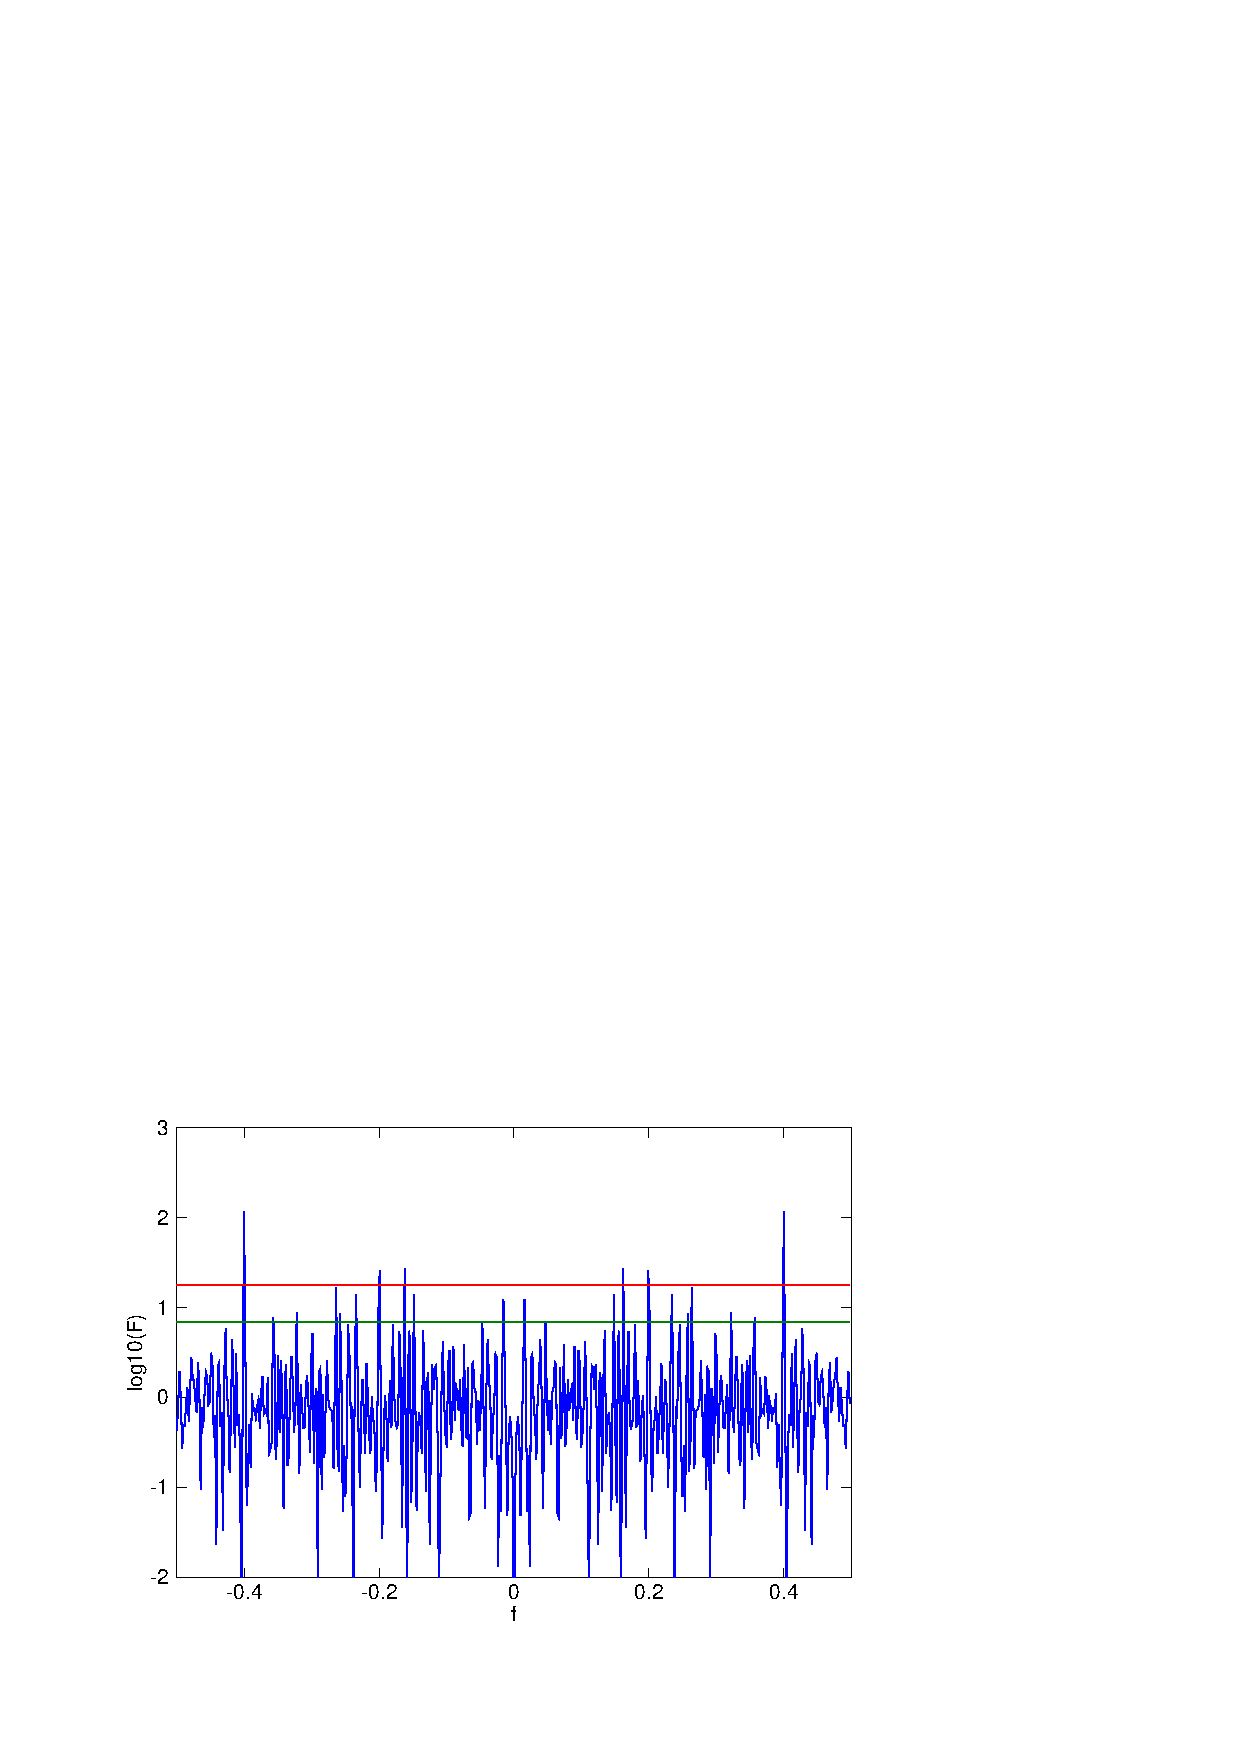
\includegraphics[width=4.75in]{pics/Fstat1_256.pdf}\\ 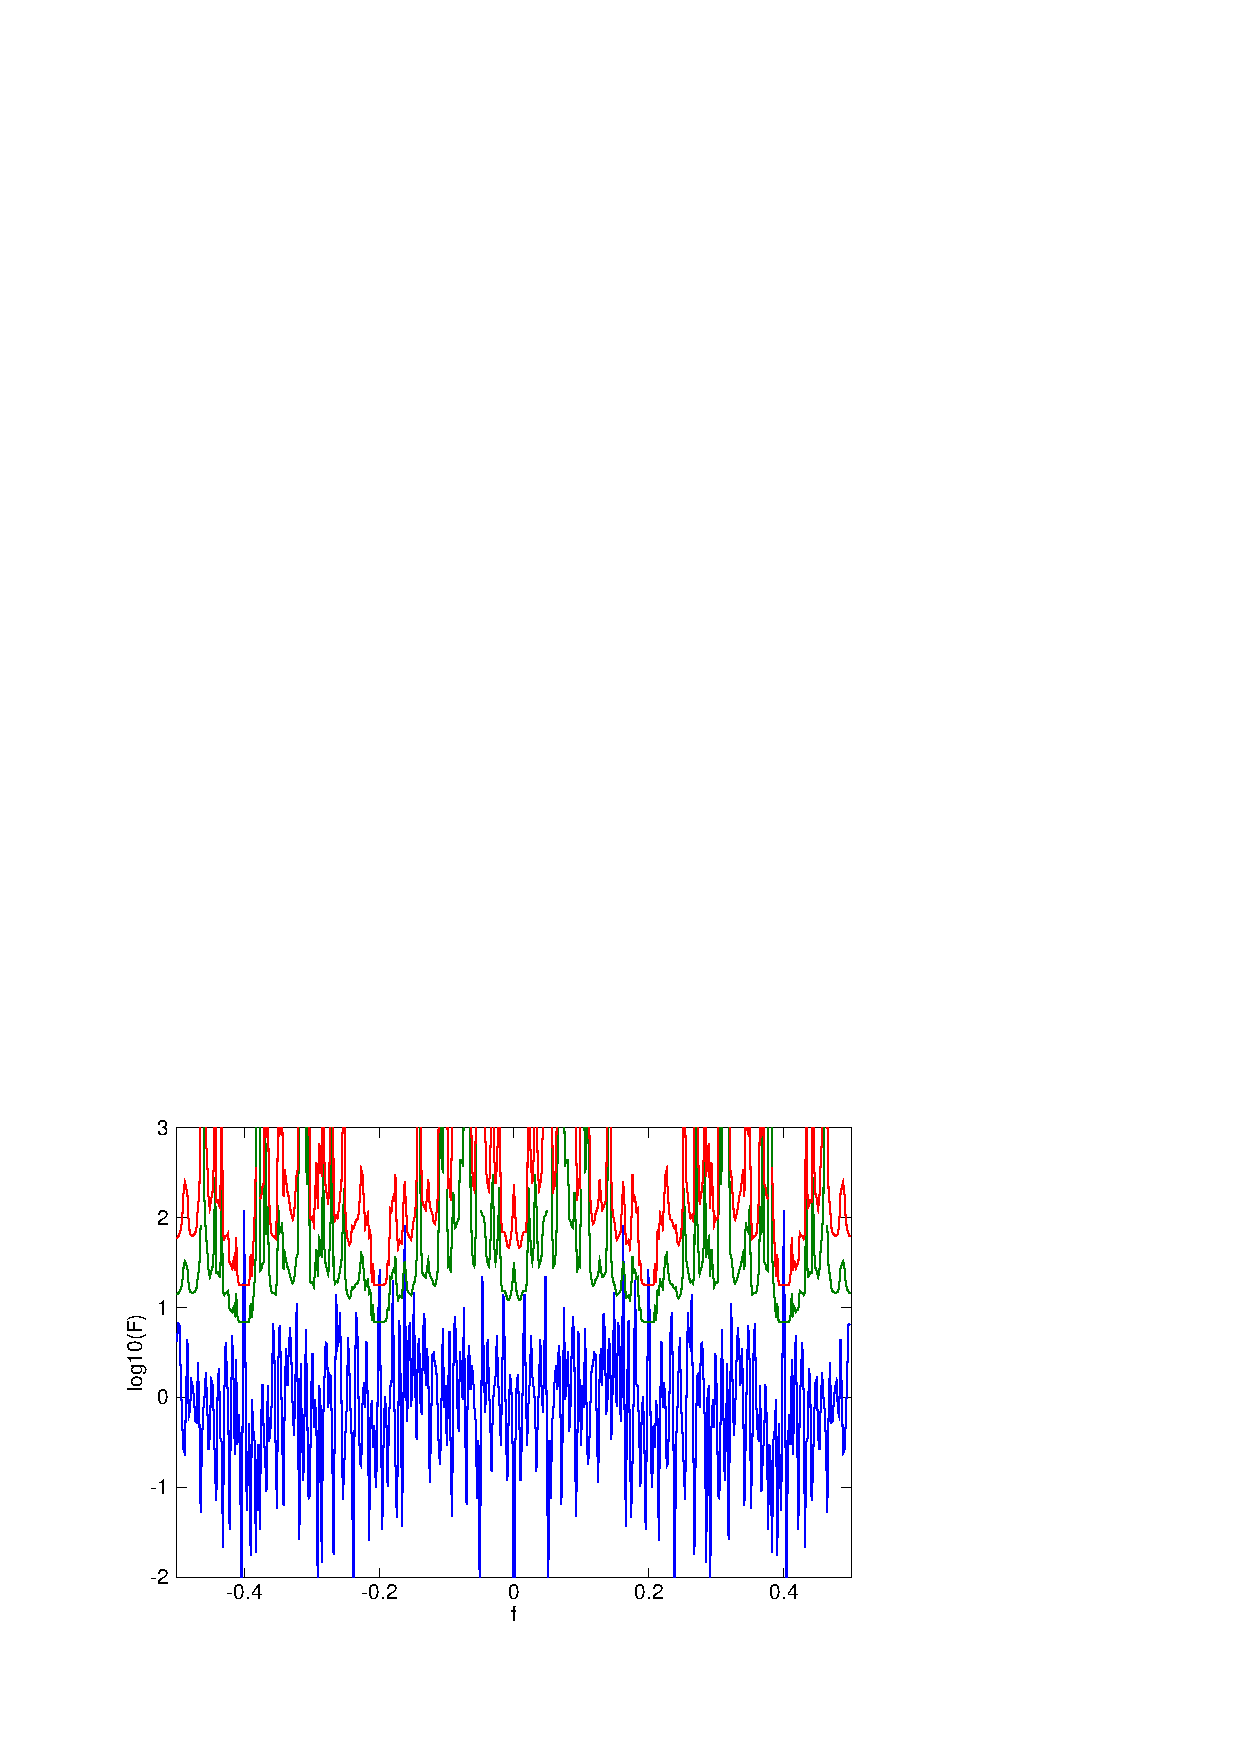
\includegraphics[width=4.75in]{pics/Fstat2_256.pdf}\\
    \caption[F-test example]{F-test at the \textcolor{green!40!black}{$p_1=95\%$} and \textcolor{red!80!black}{$p_2=99\%$} significance levels for $x(t)=\sin(2\pi0.2t)+\cos(2\pi0.4t) + \eta(t)$, where $n=256$, $nW=2$, $K=3$, and $\sigma_\eta=0.1$. The top results are eigenvalue weighted, and the bottom adaptive.\label{fig:f_stat}}
\end{figure}

For equal and eigenvalue weights, the number of degrees of freedom is constant across all frequencies.  This means $F_u$ is also constant.  For adapted weights, $F_u$ is frequency dependent, which can make a visual interpretation of the F-test more difficult.  Examples of F-tests are shown in Figure \ref{fig:f_stat}.  Notice that when adaptive weighting is used, the threshold dips down at the four frequencies $f=\pm 0.2, \pm0.4$.  This is due to the increase in degrees of freedom at these frequencies.  At the 95\%  significance level, the adaptively-weighted F-test only gives false positives at $\pm 0.16$Hz, whereas the eigenvalue-weighted F-test has 18 false positives.  At the 99\% significance level, the adaptively-weighted F-test finds only the four significant frequencies, while the eigen-value weighted one still has false positives at $\pm 0.16$Hz.

One final note: if $w_k$ is replaced with $1/K$ in all the equations in this section, the results from Percival and Walden are recovered.
\index{F-test|)}

\pagebreak

\subsection{Computing the DPSSs \label{sec:dpsscalc}}

As described in Section \ref{sec:tapers}, the discrete prolate spheroidal sequences have a fixed length $n$ and maximize the concentration problem
\begin{align*}
    \lambda = \alpha^2(h) = \dfrac{\int_{-W}^W \|\mathcal{F}(h)(f)\|^2df}{\int_{-1/2}^{1/2} \|\mathcal{F}(h)(f)\|^2 df}. \tag{\ref{eq:conc}}
\end{align*}
By applying the discrete Fourier transform, Equation \eqref{eq:conc} can be re-written in a discrete form:
\begin{align*}
    \lambda & = \left(\sum_{t=0}^{n-1}\|h(t)\|^2\right)^{-1}\sum_{t=0}^{n-1}\sum_{\tau=0}^{n-1} h(t)h(\tau)\dfrac{\sin\left[2\pi W(t-\tau)\right]}{\pi(t-\tau)}.
\end{align*}
The sequence $\{h(t)\}$ that maximizes this quantity satisfies
\begin{align}
    \sum_{\tau=0}^{n-1} \dfrac{\sin\left[2\pi W(t-\tau)\right]}{\pi(t-\tau)} h(\tau) & = \lambda h(t), \quad t=0,1,\ldots,n-1,
\end{align}
which is readily seen as the eigenvalue problem:
\begin{align}
    A h & = \lambda h, \quad \text{where }A_{ij} = \dfrac{\sin\left[2\pi W(i-j)\right]}{\pi(i-j)}. \label{eq:eigen}\index{discrete prolate spheroidal sequence (DPSS)!eigenvalue problem}\index{eigenvalues}\index{eigenvectors}
\end{align}
This produces $n$ orthonormal sequences, with eigenvalues that correspond to their concentration of energy in the normalized frequency range $[-W,W]$.  

Solving Equation \eqref{eq:eigen} can be difficult since the eigenvalues are so closely bunched together: the first $\lfloor 2nW \rfloor-1$ eigenvalues are very close to one, and the last $n-\lfloor 2nW \rfloor-1$ are clustered near zero.  This makes the problem numerically ill-conditioned.  Slepian \cite{slepian:seq} noticed that the eigenvectors satisfy a second set of equations:
\begin{align}
    \begin{gathered}
        u(t-1) h(t-1) + d(t) h(t) + u(t) h(t+1) = \theta h(t), \quad t=0,1,\ldots,n-1,\\
        u(t) = \dfrac{(t+1)(n-t-1)}{2}, \quad d(t)  = \left(\dfrac{n-1-2t}{2}\right)^2\cos(2\pi W).
    \end{gathered}\label{eq:tridiag}\index{discrete prolate spheroidal sequence (DPSS)!tridiagonal formulation}
\end{align}
Not only is this new eigenvalue problem much simpler to solve due to its symmetric tridiagonal structure, but the new eigenvalues ($\theta_k$) have a much better spread \cite{thomson:lecture}.  Thus, the discrete prolate spheroidal sequences can be computed using the system in Equation \ref{eq:tridiag}, and the energy concentrations recovered by then solving for $\lambda$ using Equation \ref{eq:eigen}:
\begin{align}
    \lambda & = \dfrac{h^\text{T}Ah}{\|h\|^2}. \label{eq:eigenvalue}
\end{align}


There are other ways of solving for the DPSSs, including Gaussian quadrature techniques \cite{thomson:multitaper}, and inverse iteration methods \cite{percival:multitaper}.  However, the tridiagonal matrix method is incredibly fast, stable, and accurate, and is the one recommended by Thomson \cite{thomson:lecture}.

\subsubsection{Even-Odd Splitting \label{sec:splitting}}

The doubly-symmetric nature of the systems in \eqref{eq:eigen} and \eqref{eq:tridiag} cause the even eigenvectors $\{h_0,h_2,\ldots\}$ to be even functions about their centre, and the odd eigenvectors $\{h_1,h_3,\ldots\}$ to be odd functions.  This means that only the first $\lceil n/2 \rceil$ elements of the vectors need to be calculated.  This allows the problem to be split in two: one for even sequences, where $h(i)=h(n-1-i)$, and one for odd, $h(i)=-h(n-1-i)$ \cite{slepian:compute}.  The tridiagonal matrices for the subproblems are described as follows:\index{discrete prolate spheroidal sequence (DPSS)!even-odd splitting}
\begin{align*}
       & \qquad\text{Even}\ n &  &\qquad\text{Odd}\ n\\[0.3em]
    d_e(i) & = d(i),\quad i=0,\ldots,\tfrac{n}{2}-2 &               d_e(i) & = d(i),\quad i=0,\ldots,\tfrac{n+1}{2}\\
    d_e(\tfrac{n}{2}-1) & = d(\tfrac{n}{2}-1)+u(\tfrac{n}{2}-1) &   u_e(i) & = u(i), \quad i=0,\ldots,\tfrac{n-3}{2}\\
    u_e(i) & = u(i), \quad i=0,\ldots,\tfrac{n}{2}-2 &              u_e(\tfrac{n-1}{2}) & = \sqrt{2}\,u(\tfrac{n-1}{2})\\
    \\
    d_o(i) & = d(i),\quad i=0,\ldots,\tfrac{n}{2}-2 &               d_o(i) & = d(i),\quad i=0,\ldots,\tfrac{n-1}{2}\\
    d_o(\tfrac{n}{2}-1) & = d(\tfrac{n}{2}-1)-u(\tfrac{n}{2}-1) &   u_o(i) & = u(i),\quad i=0,\ldots,\tfrac{n-3}{2}\\
    u_o(i) & = u(i), \quad i=0,\ldots,\tfrac{n}{2}-2
\end{align*}
where subscripts $e$ and $o$ represent entries for the even and odd subproblems, respectively.  Note that for $n$ odd, a factor $\sqrt{2}$ is necessary to maintain symmetry.  As a result, the centre value must be rescaled when constructing the final sequences: $h(\tfrac{n-1}{2})=\sqrt{2}\,h_e(\tfrac{n-1}{2})$.

Splitting into even and odd subproblems reduces memory requirements, increases computation speed, and also increases the stability of the algorithm: the eigenvalues of the new systems are now separated twice as far as the original, allowing for improvements in accuracy \cite{thomson:lecture}.